\section{Harmonic distortion}

In this section the amount of harmonic distortion of the loudspeaker is analysed, to examine if it is possible to determine the performance of the loudspeaker from harmonics. To analyse the harmonic distortion a spectrogram is used. The spectrogram is a three dimensional plot which shows the frequency, time and magnitude. Basically the spectrogram is an array of multiple FFT each calculated at a given time with a given window.

The advantages of using a spectrogram is that it gives a good overview of the spectral content in the signal at any given time. Since the harmonic frequencies depends on the fundamental frequency, it is better to use a spectrogram rather than a regular FFT, since the spectrogram will reveal all harmonic distortion for all fundamental frequency from 10 Hz to 2.4 kHz. The spectrograms for microphone in dataset 1 and 19 are shown in \autoref{fig:spec_mic}.

\begin{figure}[H]
\centering
\begin{subfigure}[t]{0.47\textwidth}
	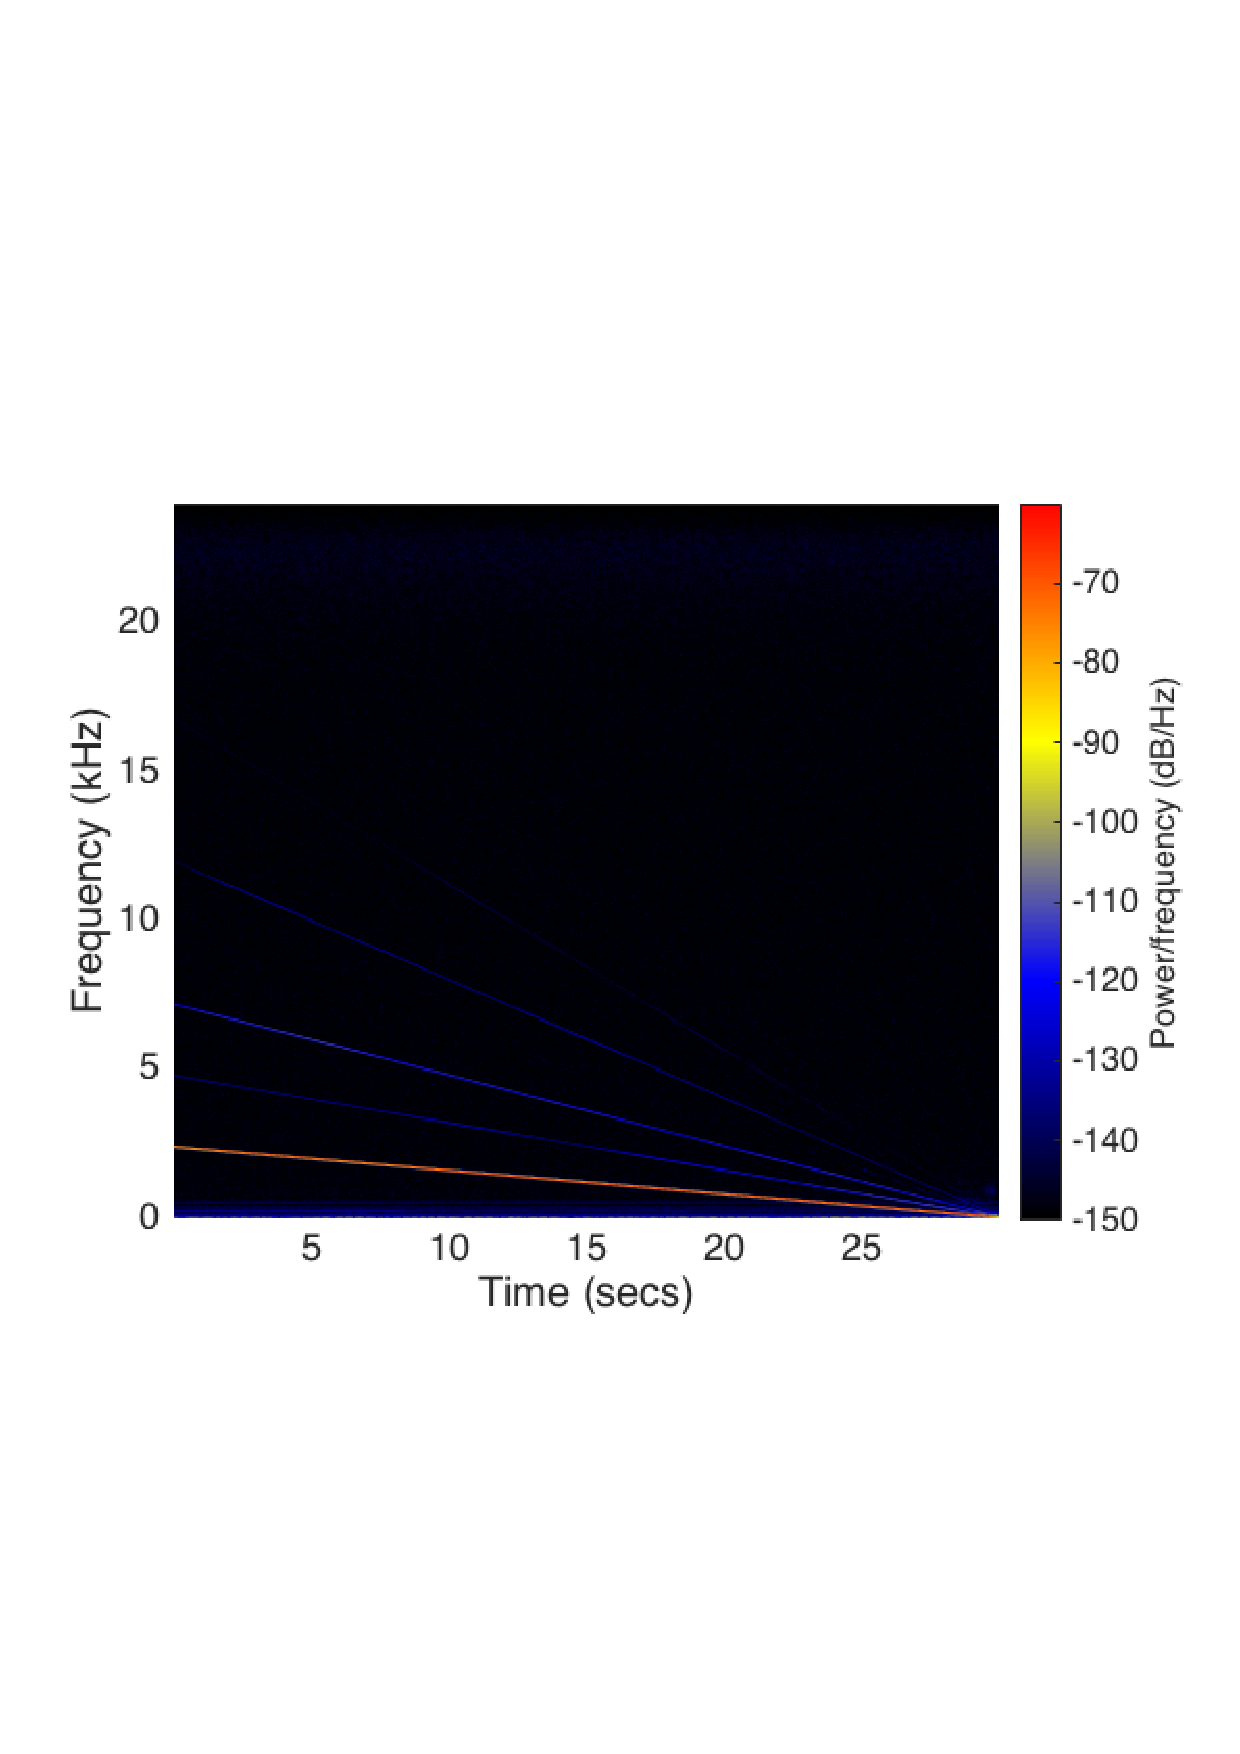
\includegraphics[width=1\textwidth]{figures/spectrogram_mic1.pdf}
	\caption{Microphone dataset 1.}
	\label{fig:spectrogram_mic1}
\end{subfigure}
\begin{subfigure}[t]{0.47\textwidth}
	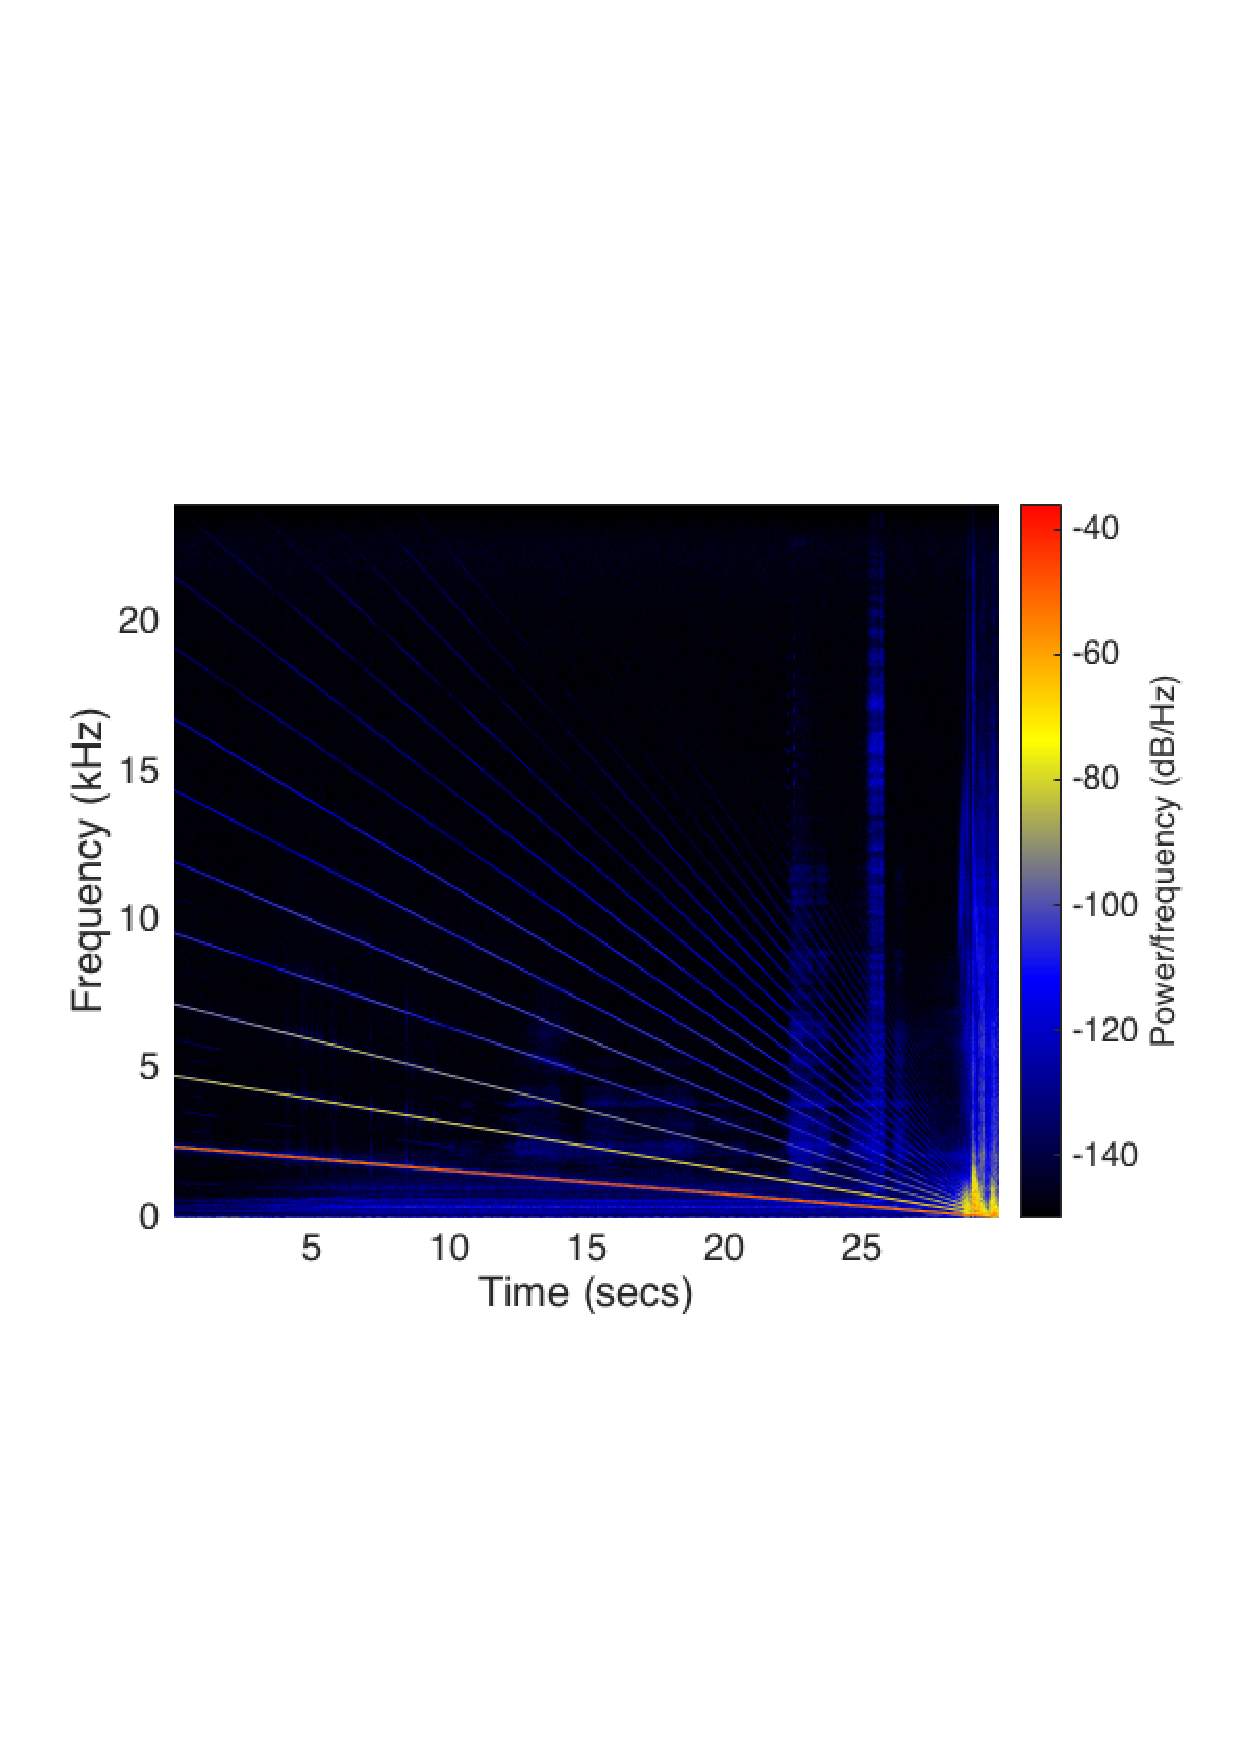
\includegraphics[width=1\textwidth]{figures/spectrogram_mic19.pdf}
	\caption{Microphone dataset 19.}
	\label{fig:spectrogram_mic19}
\end{subfigure}
\caption{The spectrograms of the microphone dataset 1 and 19. The prominent red line is the sine sweep from 2.4 kHz to 10 Hz while the yellow and blue lines along the red line are harmonic distortion.}
\label{fig:spec_mic}
\end{figure} 

The spectrograms of dataset 1 and 19, seen in \autoref{fig:spectrogram_mic1} and \autoref{fig:spectrogram_mic1}, show a prominent red line and three weak blue lines above the red line. It is seen that the red line is a linear decreasing function from 2.4 kHz to 10 Hz where the frequency is a function of time. This indicates that the red line is the fundamental frequency of the sine sweep from 2.4 kHz to 10 Hz. The blue and yellow line are linear functions of the harmonic distortions. The spectrograms clearly show that increasing the gain will increase the amount of harmonic distortion as well. An interesting observation is the spectral frequency leak that occurs at low frequency. 


\begin{figure}[H]
\centering
\begin{subfigure}[t]{0.47\textwidth}
	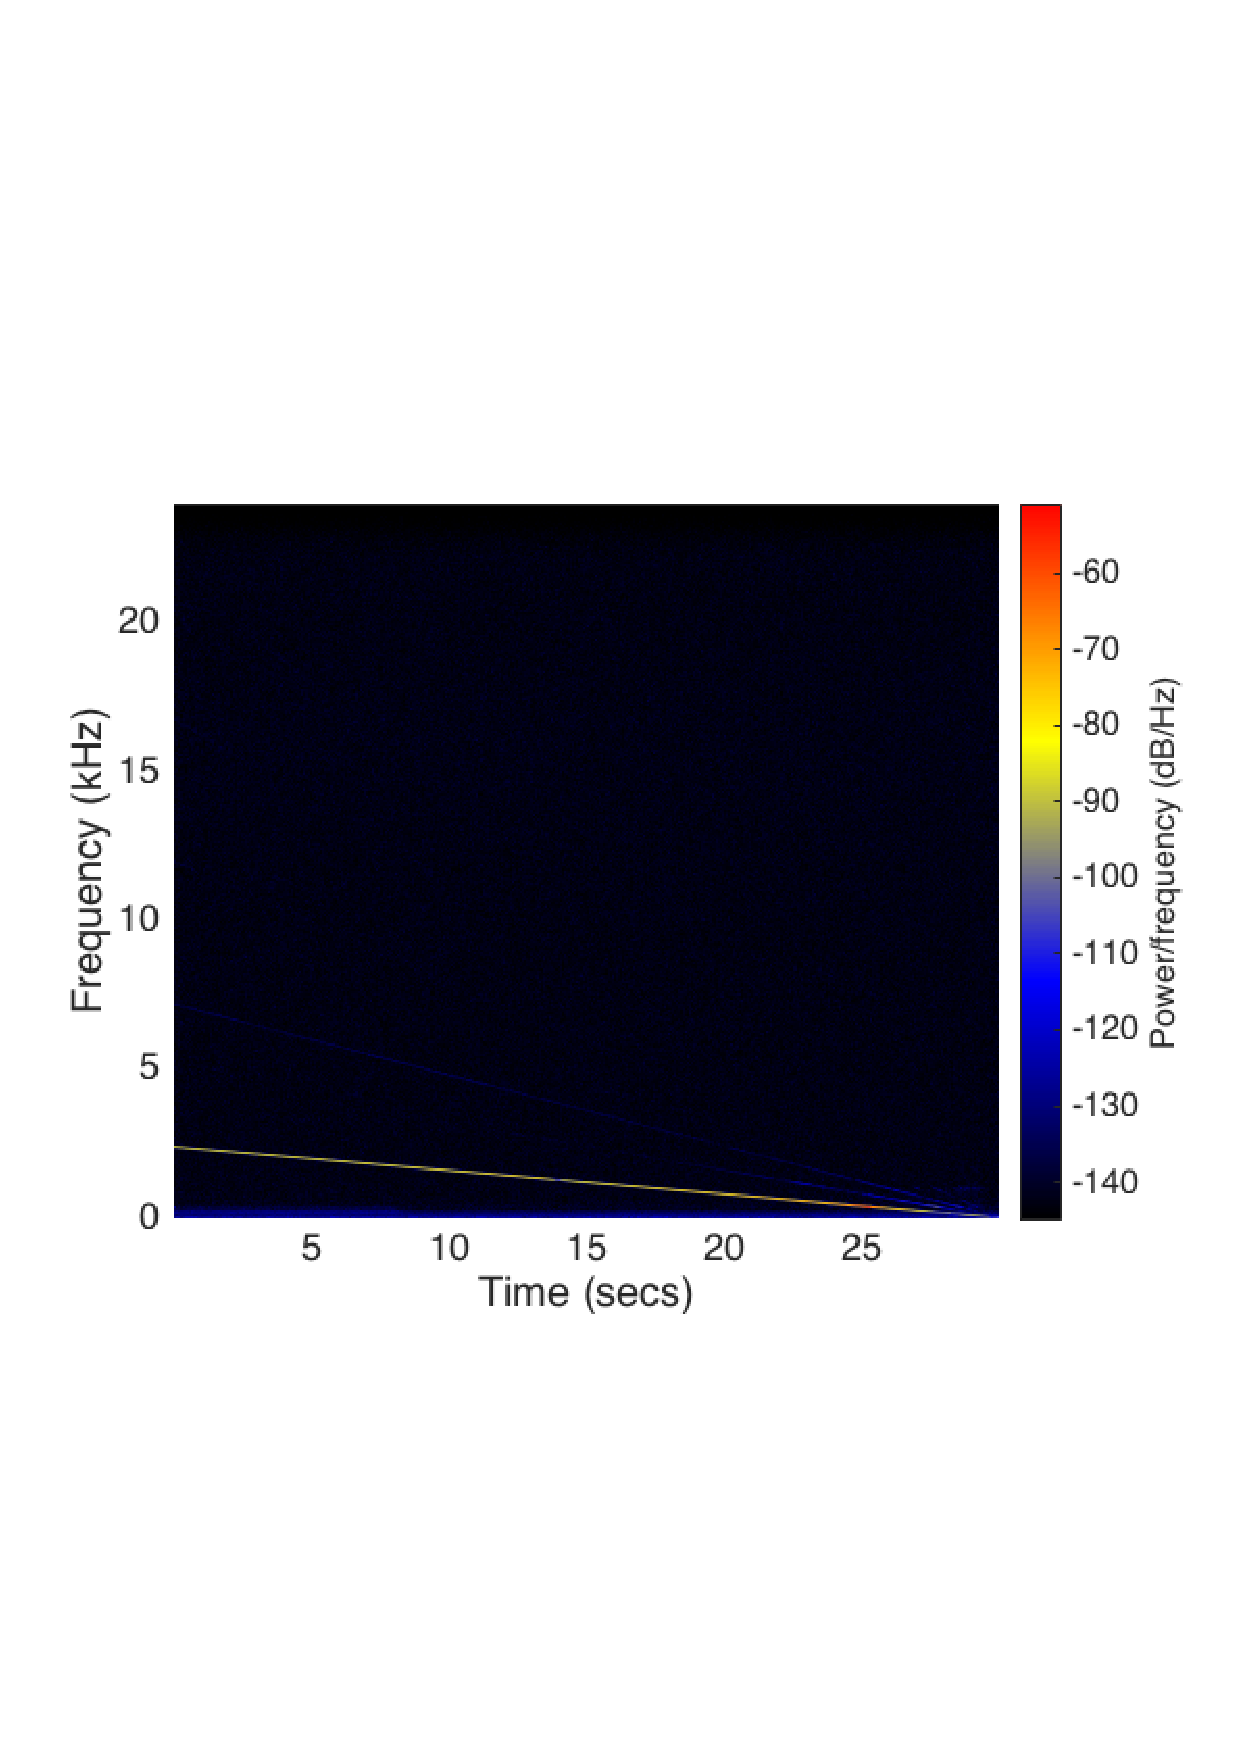
\includegraphics[width=1\textwidth]{figures/spectrogram_driver1.pdf}
	\caption{Vibration from driver.}
	\label{fig:spectrogram_driver1}
\end{subfigure}
\begin{subfigure}[t]{0.47\textwidth}
	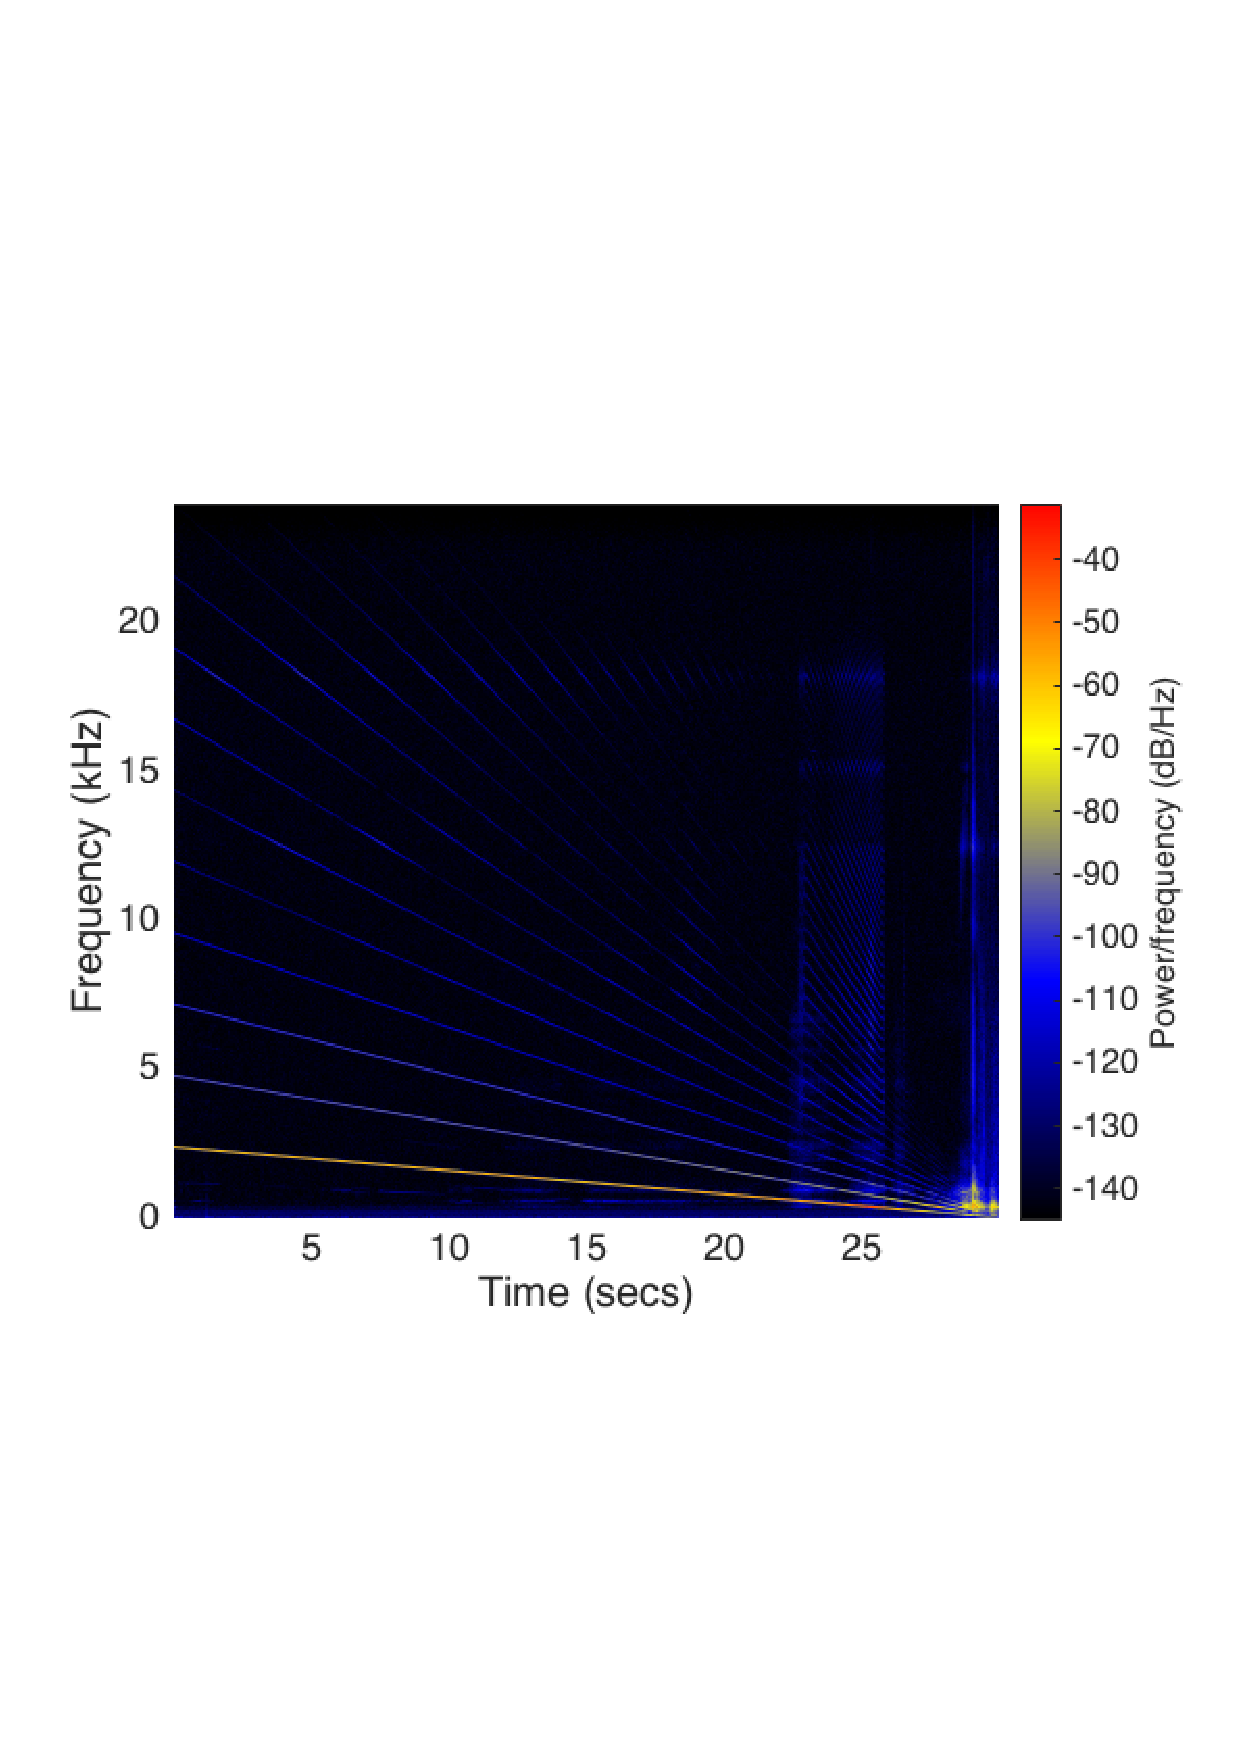
\includegraphics[width=1\textwidth]{figures/spectrogram_driver19.pdf}
	\caption{Vibration from driver.}
	\label{fig:spectrogram_driver19}
\end{subfigure}
\caption{The measured data of (a) the vibration on the driver, (b) the vibration on the enclosure, and (c) the sound pressure from the microphone. Dataset 20.}
\label{fig:spec_driver}
\end{figure} 





















